\documentclass[12pt, twoside]{article}
\usepackage[letterpaper, margin=1in, headsep=0.5in]{geometry}
\usepackage[english]{babel}
\usepackage[utf8]{inputenc}
\usepackage{amsmath}
\usepackage{amsfonts}
\usepackage{amssymb}
\usepackage{tikz}
\usetikzlibrary{quotes, angles}
\usepackage{graphicx}
%\usepackage{pgfplots}
%\pgfplotsset{width=10cm,compat=1.9}
%\usepgfplotslibrary{statistics}
%\usepackage{pgfplotstable}
%\usepackage{tkz-fct}
%\usepackage{venndiagram}
\usepackage{multicol}


\usepackage{fancyhdr}
\pagestyle{fancy}
\fancyhf{}
\fancyhead[RE]{\thepage}
\fancyhead[RO]{\thepage \\Name: \hspace{4cm} \, \\}
\fancyhead[LO]{BECA / Dr. Huson / Geometry 10th Grade\\* Unit 5: Transformation, dilation, and scale \\ 21 November 2019}

\renewcommand{\headrulewidth}{0pt}

\begin{document}
\subsubsection*{5.10b Do Now: Composition of two transformations}
  \begin{enumerate}

  \item After a dilation with center $(0,0)$, the image of $\overline{MN}$ is $\overline{M'N'}$. If $MN=4.5$ and $M'N'=18$, find the scale factor of this dilation. \vspace{3cm}

  \item In the diagram below, $\triangle ABC$ with sides of 13, 15, and 16, is mapped onto $\triangle DEF$ by a rigid motion. \\*[0.25cm]
  If $DE=2x-1$, what is the value of $x$? 
      \begin{flushright}
        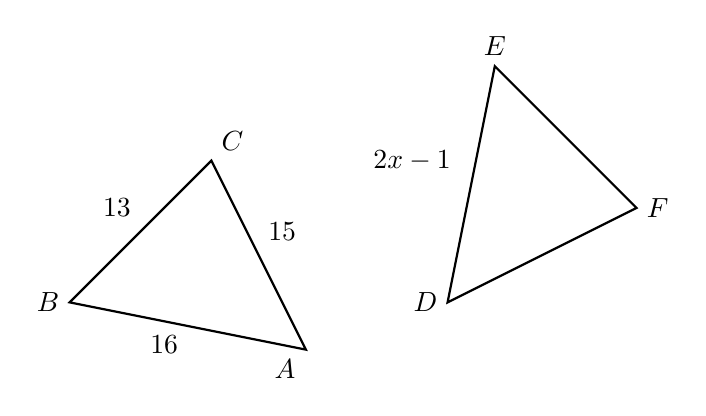
\begin{tikzpicture}[scale=.6]
          %\draw [thick, <->] (-7.4,0) -- (10.4,0) node [right] {$x$};
          %draw [thick, <->] (0,-5.4)--(0,10.4) node [above] {$y$};
          %\fill (0,0) circle[radius=0.1] node[right]{$P$};
          \draw [thick]
            (-2,1) node[below left] {$A$}--
            (-7,2) node[left] {$B$}--
            (-4,5) node[above right] {$C$}--cycle;
            \node at (-5,1.5)[below]{16};
            \node at (-6,4){13};
            \node at (-2.5,3.5){15};
            \node at (0.25,5){$2x-1$};
          \draw [thick]
            (1,2) node[left] {$D$}--
            (2,7) node[above] {$E$}--
            (5,4) node[right] {$F$}--cycle;
        \end{tikzpicture}
      \end{flushright}
    \vspace{2cm}

  \item In right triangle $ABC$ shown below, point $D$ is on $\overline{AB}$ and point $E$ is on $\overline{BC}$ such that $\triangle ABC \sim \triangle DBE$. \\*[0.25cm]
  If $AB=15$, $BC=12$, and $EC=7$, what is the length of $\overline{BD}$?
    \begin{flushright}
      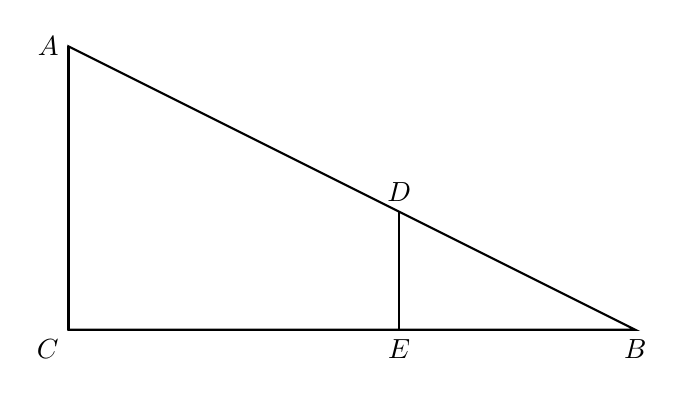
\begin{tikzpicture}[scale=0.6]
        \coordinate [label=left:$A$](A) at (-12,6);
        \coordinate [label=below:$B$](B) at (0, 0);
        \coordinate [label=below left:$C$](C) at (-12,0);
        \coordinate [label=above:$D$](D) at (-5, 2.5);
        \coordinate [label=below:$E$](E) at (-5,0);
        \draw [thick] (A)--(B)--(C)--cycle;
        \draw [thick] (A)--(C);
        \draw [thick] (D)--(E);
      \end{tikzpicture}
    \end{flushright}
    
  
\newpage

  \item Line segment $A'B'$, having a length of 12.8 cm, is the image of $\overline{AB}$ after a dilation of $\displaystyle \frac{1}{2}$ centered at the origin. What is the length of $\overline{AB}$? \vspace{4cm}
  

  \item Given two parallel lines and a transversal, as shown below.
  \begin{center}
  \begin{tikzpicture}
    \draw [<->, thick] (1,2)--(9,2);
    \draw [<->, thick] (0,0)--(8,0);
    \draw [<->, thick] (4,-1)--(5.5,3);
    \node at (4.5,0.3) [left]{$5$};
    \node at (4.5,0.3) [right]{$6$};
    \node at (4.3,-0.3) [left]{$7$};
    \node at (4.3,-0.3) [right]{$8$};
    \node at (5.2,2) [above left]{$1$};
    \node at (5.2,2) [above right]{$2$};
    \node at (5,2) [below left]{$3$};
    \node at (5,2) [below right]{$4$};
  \end{tikzpicture}
  \end{center}
  \begin{enumerate}
    \item State the angle corresponding with $\angle 6$. \vspace{0.5cm}
    \item Why does $m\angle 5 + m\angle 6 =180^\circ$? (justify) \rule{6cm}{0.15mm} \vspace{0.5cm}
    \item Why does $m\angle 7 = m\angle 2$?  (justify) \rule{7cm}{0.15mm} \vspace{0.5cm}
    \item Given $m\angle 3 = 73^\circ$ and $m\angle 5 = (3x-1)^\circ$. Find $x$. \vspace{5cm}
  \end{enumerate}

\newpage
  \item A translation maps $D(2,4) \rightarrow D'(-3,4)$. What is the image of $E(5,-5)$ under the same translation?  \vspace{3.5cm}

  \item The image of triangle $ABC$ after a translation is $\triangle A'B'C'$. Is the area of the triangle greater, smaller, or the same after the translation? Justify your answer. \vspace{3.5cm}

  \item The triangle $ABC$, shown below, undergoes a rigid motion carrying it onto triangle $XYZ$. State the transformation. (be specific)
    \begin{flushright}
      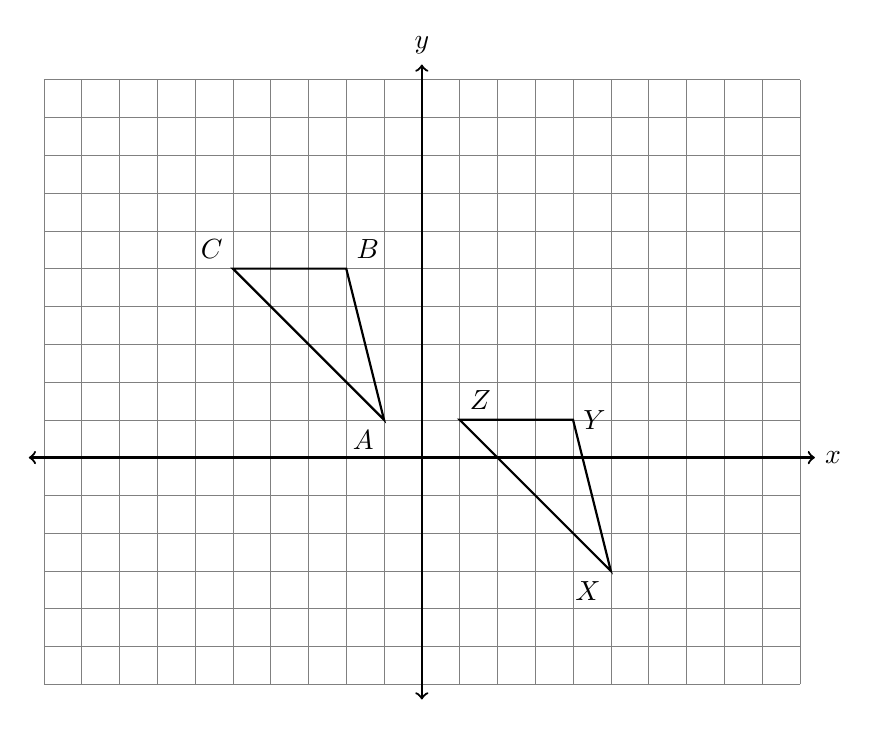
\begin{tikzpicture}[scale=.48]
        \draw [help lines] (-10,-6) grid (10,10);
        \draw [thick, <->] (-10.4,0) -- (10.4,0) node [right] {$x$};
        \draw [thick, <->] (0,-6.4)--(0,10.4) node [above] {$y$};
        \draw [thick]
          (5,-3) node[below left] {$X$}--
          (4,1) node[right] {$Y$}--
          (1,1) node[above right] {$Z$}--cycle;
        \draw [thick]
          (-1,1) node[below left] {$A$}--
          (-2,5) node[above right] {$B$}--
          (-5,5) node[above left] {$C$}--cycle;
      \end{tikzpicture}
    \end{flushright}

\newpage

\item Triangle $\triangle ABC$ is graphed on the set of axes below. The vertices of $\triangle ABC$ have the coordinates $A(2,-3)$, $B(8,1)$, and $C(-1,8)$. \\*[0.25cm]
Translate the triangle three units to the left and down one unit. Write down its coordinates in a table and plot and label it on the graph.
    \begin{flushright} %4 quadrant regents grid
    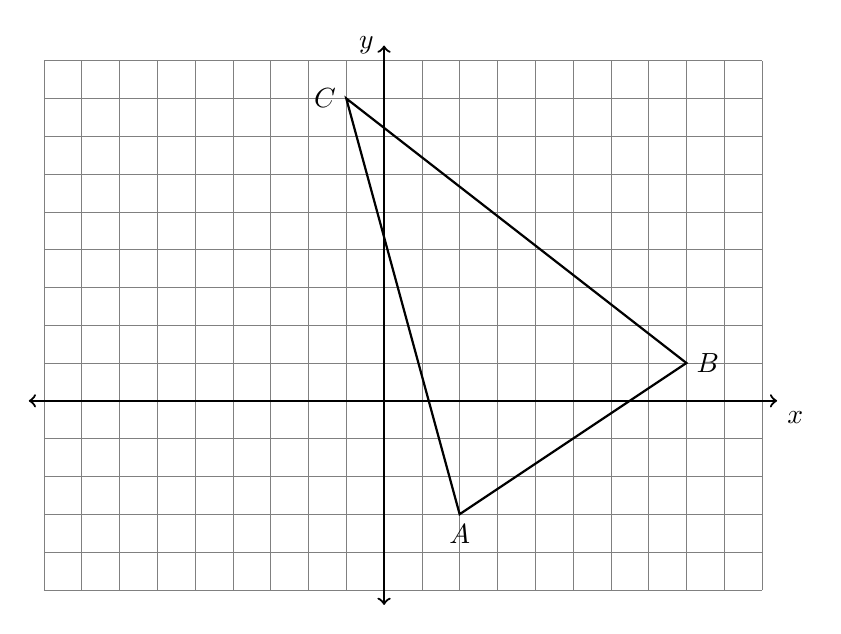
\begin{tikzpicture}[scale=.48]
      \draw [help lines] (-9,-5) grid (10,9);
      \draw [thick, <->] (-9.4,0) -- (10.4,0) node [below right] {$x$};
      \draw [thick, <->] (0,-5.4)--(0,9.4) node [left] {$y$};
      \draw [thick] (2,-3) node[below] {$A$}--
      (8,1) node[right] {$B$}--
      (-1,8) node[left] {$C$}--
      cycle;
      %\draw [fill] (5,0) circle [radius=0.1] node[above left] {$P$};
    \end{tikzpicture}
    \end{flushright}
  
\item In  $\triangle ABC$ shown below, side $\overline{AC}$ is extended to point $D$ with $m\angle DAB=122^\circ$, $m\angle C=(x+4)^\circ$, and $m\angle B=(4x+3)^\circ$. \\[0.25cm]
What is $m\angle BAC$?
\begin{flushright}
    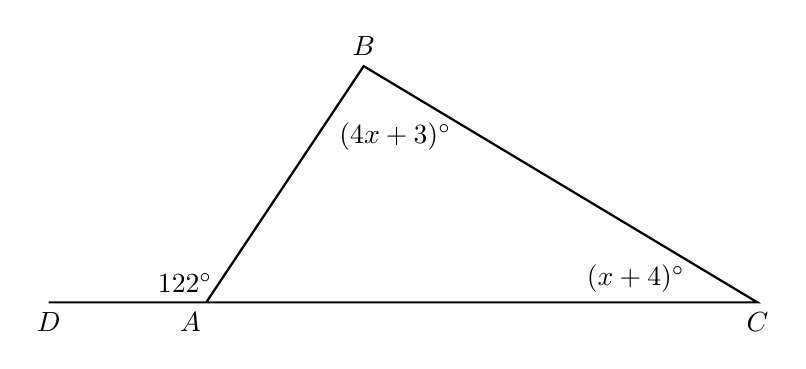
\begin{tikzpicture}
      \draw [thick](0,0)node[below]{$D$}--
        (1.8,0)node[below]{$A$}--
        (9,0)node[below]{$C$}--
        (4,3)node[above]{$B$} --(2,0);
        \node at (2.2,0)[above left]{$122^\circ$};
        \node at (8.2,0)[above left]{$(x+4)^\circ$};
        \node at (4.4,2.4)[below]{$(4x+3)^\circ$};
    \end{tikzpicture}
  \end{flushright}

\end{enumerate}
\end{document}


\item \emph{Spicy} On the set of axes below, $\triangle ABC$ has vertices at $A(-2,0)$, $B(2,4)$, $C(4,-2)$, and $\triangle DEF$ has vertices at $D(4,0)$, $E(-4,8)$, $F(-8,-4)$.
\begin{center}
  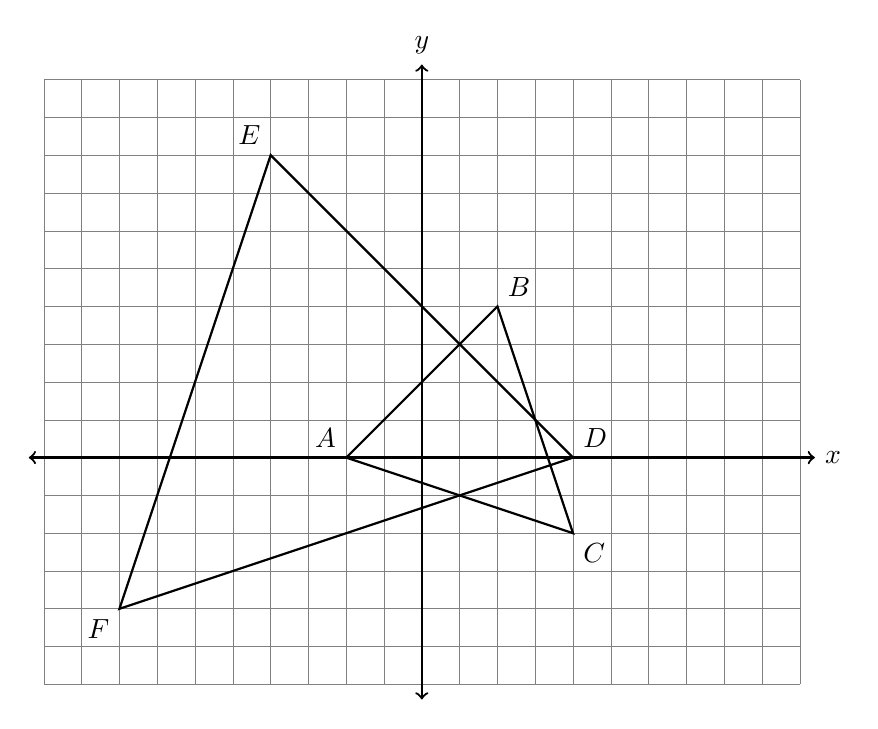
\begin{tikzpicture}[scale=.48]
    \draw [help lines] (-10,-6) grid (10,10);
    \draw [thick, <->] (-10.4,0) -- (10.4,0) node [right] {$x$};
    \draw [thick, <->] (0,-6.4)--(0,10.4) node [above] {$y$};
    \draw [thick]
      (-2,0) node[above left] {$A$}--
      (2,4) node[above right] {$B$}--
      (4,-2) node[below right] {$C$}--cycle;
    \draw [thick]
      (4,0) node[above right] {$D$}--
      (-4,8) node[above left] {$E$}--
      (-8,-4) node[below left] {$F$}--cycle;
  \end{tikzpicture}
\end{center}
Which tranformations map $\triangle ABC \rightarrow \triangle DEF$? Mark each statement True or False
  \begin{enumerate}
    \item A dilation with a scale factor of $-2$ centered at the origin \hfill True \quad False
    \item A dilation with a scale factor of $\frac{1}{2}$ centered at point $A$ \hfill True \quad False
    \item A dilation with a scale factor of 2 centered at the origin, followed by a rotation of $180^\circ$ about the origin \hfill True \quad False
    \item A dilation with a scale factor of 2 centered at the origin, followed by a reflection across the $y$-axis \hfill True \quad False
  \end{enumerate}